\documentclass[11pt,a4paper]{article}

% ===== Paquetes base =====
\usepackage[spanish,es-tabla]{babel}
\usepackage[utf8]{inputenc}
\usepackage[T1]{fontenc}
\usepackage{graphicx}
\usepackage{xcolor}
\usepackage{geometry}
\usepackage{amsmath}
\usepackage{amssymb}
\usepackage{booktabs}
\usepackage{array}
\usepackage{multirow}
\usepackage{float}
\usepackage{enumitem}
\usepackage{setspace}
\usepackage{microtype}
\usepackage{fancyhdr}
\usepackage{titlesec}
\usepackage{caption}
\usepackage[most]{tcolorbox}
\usepackage[numbers,super,sort&compress]{natbib}
\bibliographystyle{unsrtnat}

% ===== Paleta =====
\definecolor{navy}{HTML}{1B3A5C}
\definecolor{teal}{HTML}{2A9D8F}
\definecolor{brick}{HTML}{C1443C}
\definecolor{ochre}{HTML}{E9C46A}
\definecolor{lightnavy}{HTML}{EAF0F6}
\definecolor{lightteal}{HTML}{E9F6F4}
\definecolor{darkgray}{HTML}{444444}

% ===== Geometría y tipografía =====
\geometry{a4paper, top=2.6cm, bottom=2.6cm, left=2.8cm, right=2.6cm}
\setstretch{1.12}
\setlength{\parskip}{0.45em}
\setlength{\parindent}{0pt}

% ===== Encabezados =====
\titleformat{\section}{\Large\bfseries\color{navy}}{\thesection}{0.8em}{}
\titleformat{\subsection}{\large\bfseries\color{navy}}{\thesubsection}{0.7em}{}
\titleformat{\subsubsection}{\normalsize\bfseries\color{darkgray}}{\thesubsubsection}{0.6em}{}
\titlespacing*{\section}{0pt}{1.4em}{0.7em}
\titlespacing*{\subsection}{0pt}{1.1em}{0.5em}

% ===== Cabecera / pie =====
\pagestyle{fancy}
\fancyhf{}
\fancyhead[L]{\small\color{darkgray}AI Justicia --- Whitepaper técnico}
\fancyhead[R]{\small\color{darkgray}Agosto 2026}
\fancyfoot[C]{\small\thepage}
\renewcommand{\headrulewidth}{0.4pt}
\renewcommand{\headrule}{\color{navy}\hrule width\headwidth height 0.4pt}

% ===== Cajas =====
\newtcolorbox{hallazgo}[1]{enhanced, colback=lightnavy, colframe=navy,
  fonttitle=\bfseries, title={#1}, boxrule=0.8pt, arc=1.5mm,
  left=2mm, right=2mm, top=1.5mm, bottom=1.5mm}
\newtcolorbox{alerta}[1]{enhanced, colback=brick!6, colframe=brick,
  fonttitle=\bfseries, title={#1}, boxrule=0.8pt, arc=1.5mm,
  left=2mm, right=2mm, top=1.5mm, bottom=1.5mm}
\newtcolorbox{tesis}{enhanced, colback=lightteal, colframe=teal,
  boxrule=0.8pt, arc=1.5mm, left=2.5mm, right=2.5mm, top=1.8mm, bottom=1.8mm}

% ===== Captions =====
\captionsetup{font={small}, labelfont={bf,color=navy}, skip=6pt}

% ===== Listas =====
\setlist[itemize]{itemsep=0.25em, leftmargin=1.5em}
\setlist[enumerate]{itemsep=0.25em, leftmargin=1.7em}

% ===== hyperref (último) =====
\usepackage[
    colorlinks=true,
    linkcolor=navy,
    citecolor=darkgray,
    urlcolor=teal,
    bookmarks=true,
    bookmarksnumbered=true,
    unicode=true
]{hyperref}
\hypersetup{
    pdftitle={AI Justicia: Hacia un modelo de lenguaje jurídico soberano para México},
    pdfauthor={Proyecto AI Justicia},
    pdfsubject={Whitepaper técnico y de viabilidad},
    pdfkeywords={IA legal, México, LLM, LegalTech, soberanía de datos, derecho mexicano}
}

\graphicspath{{figs/}}

\begin{document}

% ================= PORTADA =================
\begin{titlepage}
\pagecolor{navy}\color{white}
\vspace*{2.2cm}
{\noindent\rule{\textwidth}{1.2pt}}\\[1.6em]
{\Huge\bfseries AI Justicia\par}
\vspace{0.5em}
{\LARGE Hacia un modelo de lenguaje jurídico\\ soberano para México\par}
\vspace{1.1em}
{\large\itshape De 430M a 10B tokens de fuentes primarias mexicanas:\\ necesidad, arquitectura y viabilidad de negocio\par}
\vspace{1.6em}
{\noindent\rule{\textwidth}{1.2pt}}

\vspace{2.2cm}
{\large Whitepaper técnico --- versión 2.0\par}
\vspace{0.4em}
{\large Agosto de 2026\par}

\vfill
{\small Proyecto AI Justicia \quad$\cdot$\quad \url{https://aijusticia.mx}\par}
\vspace{0.5em}
{\small Documento de trabajo para audiencia técnica y académica. No constituye asesoría jurídica ni oferta de inversión.\par}
\end{titlepage}
\pagecolor{white}\color{black}

% ================= RESUMEN + TOC =================
% ================= RESUMEN EJECUTIVO =================
\section*{Resumen ejecutivo}
\addcontentsline{toc}{section}{Resumen ejecutivo}

La inteligencia artificial jurídica en español ---y en particular para el derecho mexicano--- se encuentra estructuralmente desatendida. Los modelos de lenguaje legales dominantes se entrenan sobre corpus angloamericanos, alucinan citas cuando se les pregunta sobre legislación mexicana y no pueden desplegarse localmente para despachos obligados al secreto profesional. La evidencia empírica disponible es contundente: los modelos generales de propósito amplio alucinan entre el 58\% y el 88\% de las respuestas a consultas jurídicas verificables,\cite{dahl2024} e incluso las herramientas jurídicas comerciales con recuperación aumentada (RAG) ---Lexis+ AI y Westlaw AI--- alucinan entre el 17\% y el 33\% de las veces.\cite{magesh2025} Ninguno de estos sistemas está anclado en fuentes primarias mexicanas.

Este whitepaper presenta \textbf{AI Justicia}, un esfuerzo integral para construir el primer sistema de IA legal soberano de México, y evalúa de manera exhaustiva su necesidad, factibilidad técnica y viabilidad de negocio. El proyecto descansa sobre tres pilares: (i) la construcción de un \textbf{corpus vivo de más de 10B tokens de fuentes primarias exclusivamente mexicanas} ---legislación federal y estatal, gacetas oficiales, jurisprudencia federal y local, y doctrina universitaria---, cuya base normativa de reutilización es sólida (el art.~14, fracc.~VII de la LFDA excluye los textos legislativos, administrativos y judiciales de la protección autoral\cite{lfda}); (ii) un \textbf{harness de generación anclada en recuperación} donde toda afirmación jurídica debe verificarse contra pasajes recuperados, con abstención honesta cuando la evidencia es insuficiente; y (iii) una \textbf{estrategia de entrenamiento soberano} para \textbf{Tlamatini} ---el modelo jurídico mexicano del proyecto, del náhuatl \emph{tlamatini}, el que sabe'': los sabios-consejeros del México central prehispánico--- que sintetiza las lecciones de SaulLM-7B (continued pretraining de dominio con replay)\cite{colombo2024} y de la generación industrial de modelos legales (CPT fuerte más fusión lineal), extendida con \emph{harness training}: enseñar el formato de respuesta con citas ancladas durante el propio preentrenamiento.

\begin{tesis}
\textbf{Tesis central.} Para IA jurídica específica de jurisdicción, la combinación de \emph{harness en los pesos} más \emph{recuperación en inferencia} supera a cualquiera de las dos estrategias por separado. El CPT de dominio produce la \emph{forma} correcta de la respuesta jurídica; la recuperación produce los \emph{hechos} correctos; el harness training los unifica. Y el costo de cómputo del run principal de CPT ---del orden de \textbf{USD 300--1,000} en GPU rentada--- es marginal frente al verdadero activo del proyecto: la ingeniería de datos sobre un corpus que ningún competidor posee.
\end{tesis}

El análisis de mercado muestra una oportunidad real y medible. El mercado LegalTech latinoamericano alcanzó USD 1.9 miles de millones en 2025 y se proyecta a USD 4.9 miles de millones en 2034 (CAGR 10.68\%),\cite{imarc2025} mientras el mercado global de servicios legales supera el billón de dólares anuales.\cite{mordorlegalservices2026} En México operan alrededor de 46,000 firmas de abogados\cite{industryresearch2026} y ejercen cerca de 449,000 abogados,\cite{mirada360} con más de 1.2 millones de egresados de derecho acumulados.\cite{forojuridico2023} La demanda ciudadana es masiva y está desatendida: la mitad de los mexicanos enfrentó un problema jurídico en los últimos dos años, pero solo 30\% buscó asesoría legal y apenas 5 de cada 100 acudieron a tribunales o policías.\cite{wjpmx2019,justiciaabierta2025} Estimamos un TAM mexicano de $\sim$USD 420M, un SAM de $\sim$USD 94M anuales en asientos profesionales, y un SOM a cinco años de USD 5--17M de ARR combinando suscripciones profesionales y despliegues soberanos on-premise.

La ventaja competitiva es defensible precisamente porque es incómoda de replicar: la regulación mexicana (LFPDPPP 2025, con la Secretaría Anticorrupción y Buen Gobierno como autoridad\cite{lfpdppp,ccn2025}) y el deber penal de secreto profesional (arts.~210--211 del CPF\cite{cpf}) hacen jurídicamente inaceptable para los despachos mexicanos subir documentos privilegiados a APIs extranjeras que pueden retener y reutilizar sus entradas. Los incumbentes globales ---Harvey (valorado en USD 11 mil millones\cite{harvey2026}), vLex Vincent, Thomson Reuters CoCounsel, Lexis+ AI--- operan exclusivamente en nube, con precios de USD 300--500 por asiento/mes,\cite{vaquill2026} y ninguno entrena sobre corpus mexicanos ni ofrece despliegue soberano. En este mercado, \textbf{el cumplimiento normativo no es una característica: es el foso defensivo}.

El documento se organiza como sigue: la Sección~\ref{sec:problema} define las tres fallas estructurales del estado del arte; la Sección~\ref{sec:necesidad} cuantifica la necesidad social y el mercado; la Sección~\ref{sec:marco} analiza el marco regulatorio que vuelve obligatoria la soberanía; la Sección~\ref{sec:relacionado} revisa el trabajo previo; las Secciones~\ref{sec:corpus} y~\ref{sec:entrenamiento} detallan el corpus y la estrategia de entrenamiento; la Sección~\ref{sec:viabilidad} presenta el modelo de negocio y sus unit economics; y las Secciones~\ref{sec:riesgos}--\ref{sec:roadmap} discuten riesgos, hoja de ruta y contribuciones.

\newpage
\tableofcontents
\newpage

% ================= CUERPO =================
% ================= 1. EL PROBLEMA =================
\section{El problema: tres fallas estructurales}\label{sec:problema}

El estado actual de la IA jurídica para México puede caracterizarse por tres fallas que se refuerzan mutuamente. Ninguna es conjetural: las tres están medidas en literatura revisada por pares o en evaluaciones propias reproducibles, y las tres apuntan a la misma conclusión arquitectónica ---un sistema legalmente usable para México debe ser \emph{anclado en fuentes mexicanas}, \emph{desplegable localmente} y \emph{alimentado por un corpus que hoy no existe}.

\subsection{Alucinación de derecho: fluida, confiada y errónea}

La literatura sobre alucinación legal es ya robusta. Dahl et al. administraron más de 200,000 consultas verificables a GPT-3.5, GPT-4, Llama 2 y PaLM 2, y encontraron tasas de alucinación entre el 58\% (GPT-4) y el 88\% (Llama 2); al responder sobre el \emph{holding} de una sentencia, los modelos alucinan al menos 75\% del tiempo.\cite{dahl2024} Dos hallazgos del estudio son especialmente relevantes para México: el desempeño \emph{empeora sistemáticamente en jurisdicciones menos prominentes} (tribunales inferiores, materias de baja cobertura), y los modelos carecen de autoconciencia del error ---refuerzan premisas jurídicas incorrectas del usuario en lugar de corregirlas.\cite{dahl2024} El derecho mexicano es, desde la perspectiva de un corpus de entrenamiento dominado por texto anglosajón, la definición exacta de una jurisdicción poco prominente.

La recuperación aumentada mitiga pero no elimina el problema. Magesh et al., en la primera evaluación prerregistrada de herramientas jurídicas comerciales con RAG, midieron tasas de alucinación de 17\% en Lexis+ AI y Ask Practical Law AI, y de 33\% en Westlaw AI-Assisted Research, frente a 43\% de GPT-4; el modo de falla más peligroso que documentan es la respuesta \emph{misgrounded}: una cita a una fuente real que no sustenta la afirmación.\cite{magesh2025,stanfordhai2024} Un ensayo controlado aleatorio con 127 estudiantes de derecho refuerza el punto desde otro ángulo: quienes usaron una herramienta RAG (Vincent AI de vLex) produjeron trabajo con una tasa de alucinación comparable a no usar IA, mientras que quienes usaron un modelo de razonamiento sin RAG produjeron mejor análisis pero introdujeron alucinaciones.\cite{ailawlibrarians2026}

Nuestra propia evaluación reproduce el fenómeno en el contexto mexicano. Sometimos un modelo legal de fundación anglosajón de última generación (referenciado en este documento como Thomson-1.0-Small, véase la Sección~\ref{sec:relacionado}) a una batería de 30 preguntas jurídicas ciudadanas canónicas ---laboral, familiar, consumidor, vivienda---. Respondió 30/30 con fluidez y 93\% de las respuestas citaban legislación. La inspección reveló errores sistemáticos de cita: atribuyó la protección contra despido por embarazo al ``art.~139 LFT'' (el correcto es el 164) y la fórmula indemnizatoria de ``3 meses más 20 días por año'' al art.~48 (es el art.~50). Para un ciudadano que no puede verificar, una cita fluida, confiada y errónea es el peor modo de falla posible: tiene la forma de certeza jurídica sin su contenido.

\begin{alerta}{Modo de falla crítico}
El CPT de dominio enseña la \emph{forma} del razonamiento jurídico ---registro, estructura, referencias institucionales--- pero no garantiza anclaje factual en un sistema jurídico específico. La alucinación de citas \textbf{sobrevive al entrenamiento de dominio}. El anclaje jurisdiccional requiere recuperación sobre fuentes primarias de esa jurisdicción.
\end{alerta}

\subsection{Dependencia de nube frente al secreto profesional}

El abogado mexicano opera bajo un deber jurídico de sigilo con sanción penal: el Código Penal Federal tipifica la revelación de secretos conocidos con motivo del empleo, cargo o puesto (art.~210) y la agrava cuando quien revela es un prestador de servicios profesionales (art.~211: uno a cinco años, multa y suspensión de profesión).\cite{cpf} A ello se suma la nueva Ley Federal de Protección de Datos Personales en Posesión de los Particulares (DOF 20 de marzo de 2025), que impone obligaciones reforzadas sobre datos sensibles ---condición típica de los expedientes jurídicos--- y regula expresamente el tratamiento automatizado de datos con implicaciones directas para sistemas de IA.\cite{lfpdppp,cosio2026}

Subir documentos privilegiados de clientes a una API de LLM extranjera ---que puede retener entradas, revisarlas con humanos o usarlas para entrenamiento, bajo jurisdicciones que además habilitan requerimientos gubernamentales foráneos--- es jurídicamente indefendible para un despacho mexicano. No es una preferencia de despliegue: es una restricción de cumplimiento. Las herramientas dominantes (Harvey, CoCounsel, Lexis+ AI, Vincent) se ofrecen exclusivamente como SaaS en nube.\cite{harvey2026,vlex2018} La apertura de regiones cloud en Querétaro por AWS y Google Cloud\cite{aws2024,gcp2024} resuelve la \emph{residencia} del dato pero no la \emph{soberanía de inferencia}: el modelo sigue siendo una caja negra operada por un tercero, con políticas de retención ajenas. La literatura sobre soberanía de IA distingue cuatro capas ---corpus, entrenamiento, lingüística e inferencia--- y coincide en que la que realmente importa a las empresas reguladas es la última: dónde corre el modelo y quién audita lo que entra y sale.\cite{alia2026} Un modelo soberano desplegable on-premise no es un lujo: es la única arquitectura compatible con el deber de sigilo.

\subsection{El corpus mexicano no existe}

SaulLM-7B se entrenó sobre 30B tokens de derecho anglosajón destilados de 94B tokens crudos;\cite{colombo2024} los modelos industriales de Thomson Reuters o Harvey descansan sobre corpus propietarios angloamericanos de decenas de miles de millones de tokens. Para México no existe equivalente ---no porque los datos no existan, sino porque están dispersos en más de 33 portales judiciales, 32 sistemas estatales de gaceta, una gaceta federal con índices desde 1917,\cite{sidof} y repositorios universitarios, la mayoría detrás de protecciones anti-bot, cadenas de tokens de sesión, bloqueos geográficos y aplicaciones legadas. La literatura de NLP jurídico en español refleja este vacío: los recursos a escala existentes (p.~ej. Legal-ES y la tarea IberLegal) cubren textos administrativos y legislativos \emph{españoles}, no mexicanos.\cite{legales2020}

La consecuencia es un círculo vicioso: sin corpus no hay entrenamiento de dominio; sin entrenamiento de dominio, los modelos alucinan el derecho mexicano; y sin anclaje, la IA jurídica es inutilizable precisamente donde más se necesita ---en un país donde la mitad de la población enfrenta problemas jurídicos y solo 5 de cada 100 llegan a una institución.\cite{wjpmx2019,justiciaabierta2025} Romper ese círculo es el objeto de este proyecto.

\begin{figure}[H]
\centering
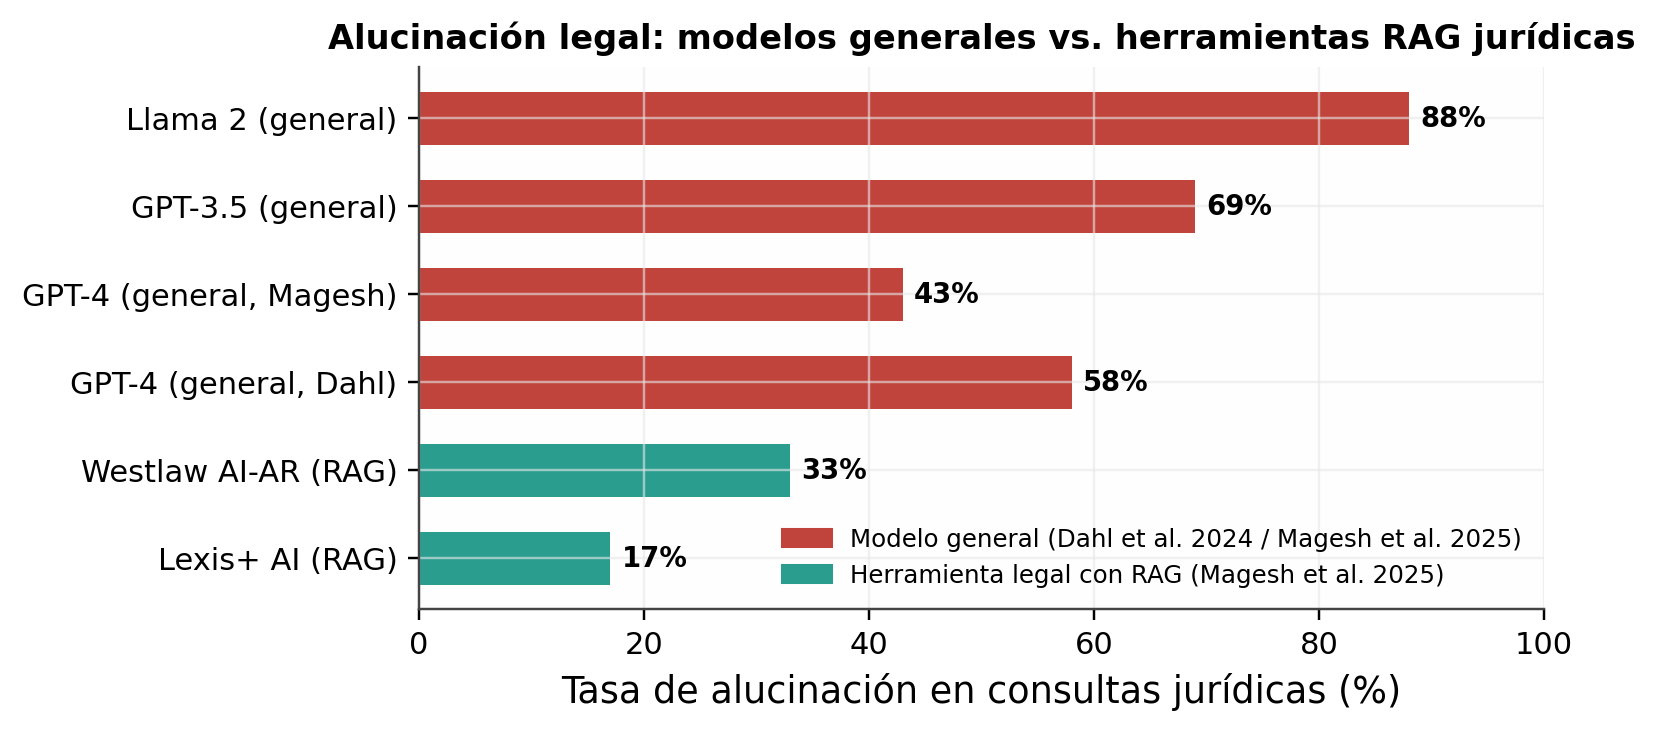
\includegraphics[width=0.92\textwidth]{fig_alucinacion.png}
\caption{Tasas de alucinación en consultas jurídicas verificables: modelos generales (58--88\%\cite{dahl2024}) frente a herramientas jurídicas comerciales con RAG (17--33\%\cite{magesh2025}). Ninguna herramienta medida está anclada en fuentes mexicanas.}
\label{fig:alucinacion}
\end{figure}

% ================= 2. NECESIDAD Y MERCADO =================
\section{La necesidad: demanda social y oportunidad de mercado}\label{sec:necesidad}

\subsection{Un déficit de acceso a la justicia de escala masiva}

La necesidad social subyacente está medida con precisión inusual. La Encuesta a Población General del World Justice Project ---más de 25,000 entrevistas en México--- documenta que los problemas con posibles consecuencias legales son un asunto cotidiano: \textbf{la mitad de los mexicanos experimentó un problema de justicia cotidiana en los últimos dos años}, desde conflictos de consumo hasta desalojos; solo \textbf{30\% buscó asesoría o representación legal}; y apenas \textbf{5 de cada 100 personas con un problema acudieron a tribunales o policías}. El 40\% reportó al menos una consecuencia negativa derivada del problema, especialmente en salud y estabilidad financiera.\cite{wjpmx2019,justiciaabierta2025} Proyectado a una población de $\sim$130 millones, esto implica del orden de \textbf{32 millones de problemas jurídicos al año}, de los cuales solo $\sim$1.6 millones tocan una institución formal.

El sistema que debería absorber esa demanda opera al límite. México cayó al lugar \textbf{121 de 143 países} en el WJP Rule of Law Index 2025 ---135 en justicia penal y 134 en ausencia de corrupción---, en un contexto global donde la justicia civil se debilitó en 68\% de los países medidos.\cite{mbn2025wjp,wjp2025} En la Ciudad de México, el número de juzgadores bajó de 486 (2023) a 425 (marzo 2025) mientras cada juez penal carga en promedio 289 causas (promedio nacional: 365); solo el paro judicial de mayo--julio de 2025 dejó sin atender $\sim$48,000 audiencias y 1.44 millones de promociones.\cite{eleconomista2025} La escasez estructural de capacidad humana es exactamente el tipo de brecha que un asistente jurídico confiable puede amortiguar ---no sustituyendo al juzgador ni al abogado, sino reduciendo el costo de información jurídica para quien hoy no puede pagarlo.

\begin{figure}[H]
\centering
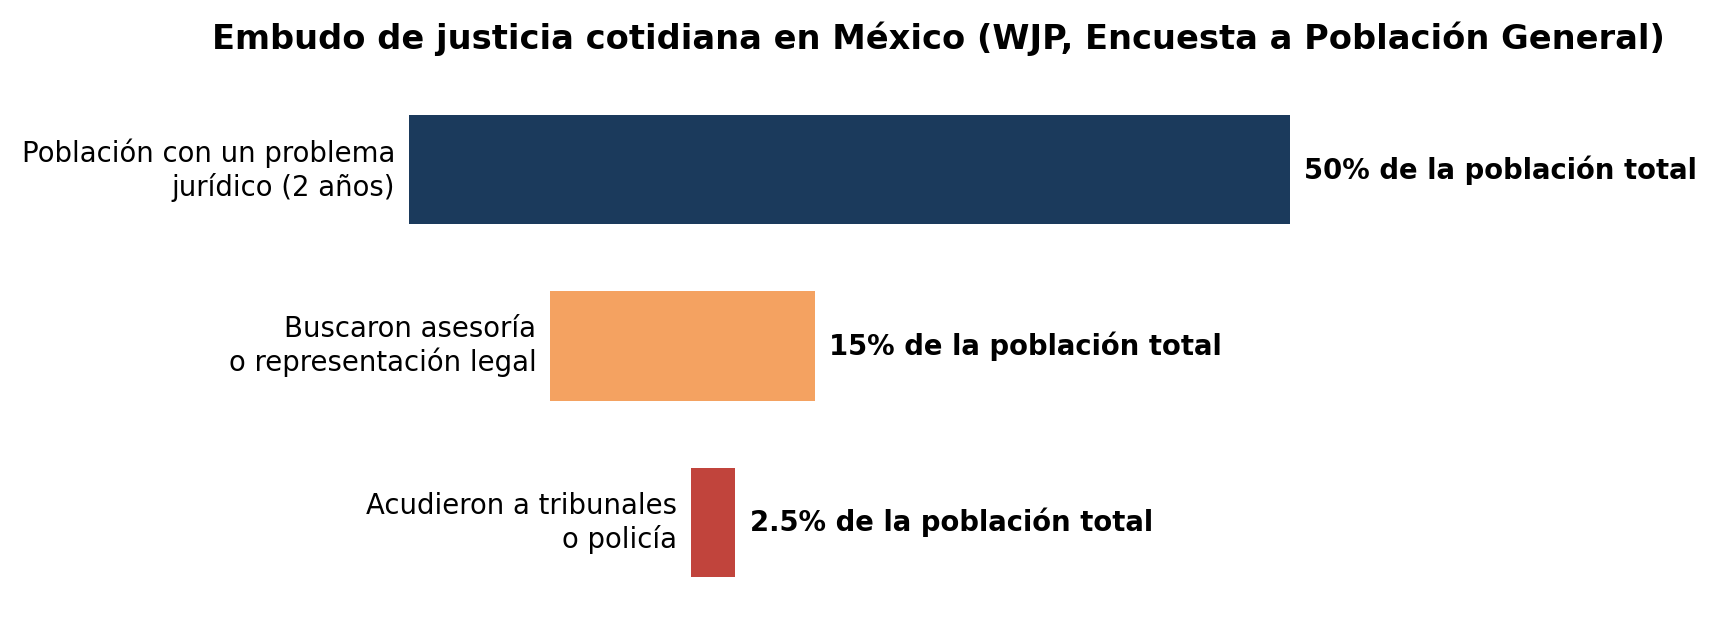
\includegraphics[width=0.86\textwidth]{fig_acceso_justicia.png}
\caption{El embudo de la justicia cotidiana en México según la Encuesta a Población General del WJP: la mitad de la población enfrenta problemas jurídicos, menos de un tercio busca asesoría y solo 5 de cada 100 llegan a tribunales o policías.\cite{wjpmx2019,justiciaabierta2025}}
\label{fig:acceso}
\end{figure}

\subsection{El mercado profesional: una abogacía numerosa y subdigitalizada}

La oferta profesional es igualmente singular. Derecho es la segunda carrera más estudiada de México, con más de \textbf{1.2 millones de egresados} acumulados y cerca de \textbf{2,000 escuelas} que la imparten;\cite{forojuridico2023} los abogados en ejercicio se estiman en $\sim$\textbf{449,000},\cite{mirada360} con un salario mensual promedio de apenas $\sim\$13,300$ MXN que concentra la mayor parte de la profesión en el segmento de despachos pequeños y práctica individual.\cite{forojuridico2023,datamexico} Operan alrededor de \textbf{46,000 firmas} en el país.\cite{industryresearch2026} Es un mercado profesional enorme en personas y atomizado en presupuesto: exactamente el perfil que no puede pagar USD 300--500 por asiento/mes de las suites anglosajonas,\cite{vaquill2026} pero sí una fracción de ese precio por una herramienta que además le resuelve el problema de cumplimiento.

La brecha de adopción tecnológica está documentada: mientras 84\% de las firmas legales globales consideran la inversión en tecnología una prioridad estratégica (Wolters Kluwer, \emph{Future Ready Lawyer}), solo 30\% de los despachos latinoamericanos se sienten preparados para el cambio; México concentra más de 25 startups legaltech, agrupadas en gestión de despachos, automatización de contratos, marketplaces legales, consultas en línea y pruebas digitales ---\textbf{ninguna construye modelos de lenguaje propios ni corpus de entrenamiento}.\cite{computerweekly2025}

\subsection{Tamaño de mercado: TAM, SAM, SOM}

El mercado LegalTech latinoamericano fue valuado en \textbf{USD 1.9 miles de millones en 2025} y se proyecta a \textbf{USD 4.9 miles de millones en 2034} (CAGR 10.68\%), impulsado por la adopción de IA y la demanda de soluciones con seguridad de datos.\cite{imarc2025} El mercado global de LegalTech se estima entre USD 34--39 mil millones (2025--2026) con proyecciones a USD 72--78 mil millones hacia 2031--2034;\cite{mordor2026,fortune2026} el mercado global de \emph{servicios} legales ---el techo último--- supera USD 1.1 billones en 2026.\cite{mordorlegalservices2026} Dos detalles de segmentación importan para nuestra estrategia: las pymes son el segmento de mayor crecimiento (CAGR 16.45\%)\cite{mordor2026} y el despliegue \emph{on-premise} conserva una participación mayoritaria proyectada ($\sim$63\% en 2026), sustentada precisamente en requisitos de control y aislamiento de la información.\cite{fortune2026}

\begin{figure}[H]
\centering
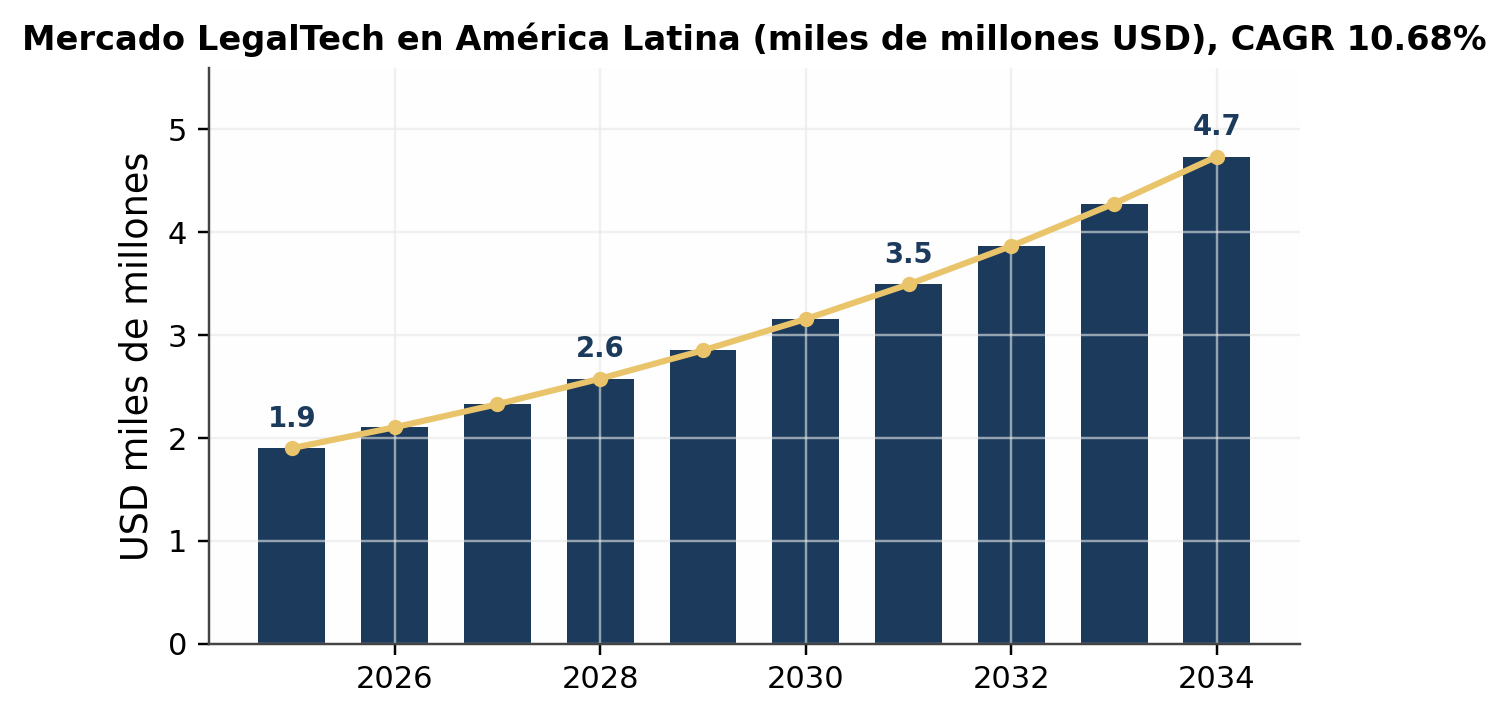
\includegraphics[width=0.88\textwidth]{fig_mercado_latam.png}
\caption{Trayectoria del mercado LegalTech latinoamericano 2025--2034 según IMARC.\cite{imarc2025}}
\label{fig:latam}
\end{figure}

Con estos parámetros construimos un dimensionamiento conservador propio (Figura~\ref{fig:tam}): atribuyendo a México $\sim$22\% del mercado latinoamericano (segunda economía de la región), el \textbf{TAM} mexicano de LegalTech es $\sim$\textbf{USD 418M} (2025). El \textbf{SAM} ---IA legal en asientos profesionales--- se estima en $\sim$\textbf{USD 94M/año}: 449,000 abogados $\times$ USD 35/asiento/mes (una décima parte del precio de las suites incumbentes) $\times$ 50\% de profesionales en práctica con capacidad de pago. El \textbf{SOM} a cinco años combina dos líneas: 3\% de penetración en asientos profesionales ($\sim$USD 5.7M ARR) y 2\% de las 46,000 firmas adoptando el tier soberano on-premise a USD 12,000/año ($\sim$USD 11M ARR), para un rango de \textbf{USD 6--17M de ARR} sin contar la línea ciudadana ni licenciamiento del corpus.

\begin{figure}[H]
\centering
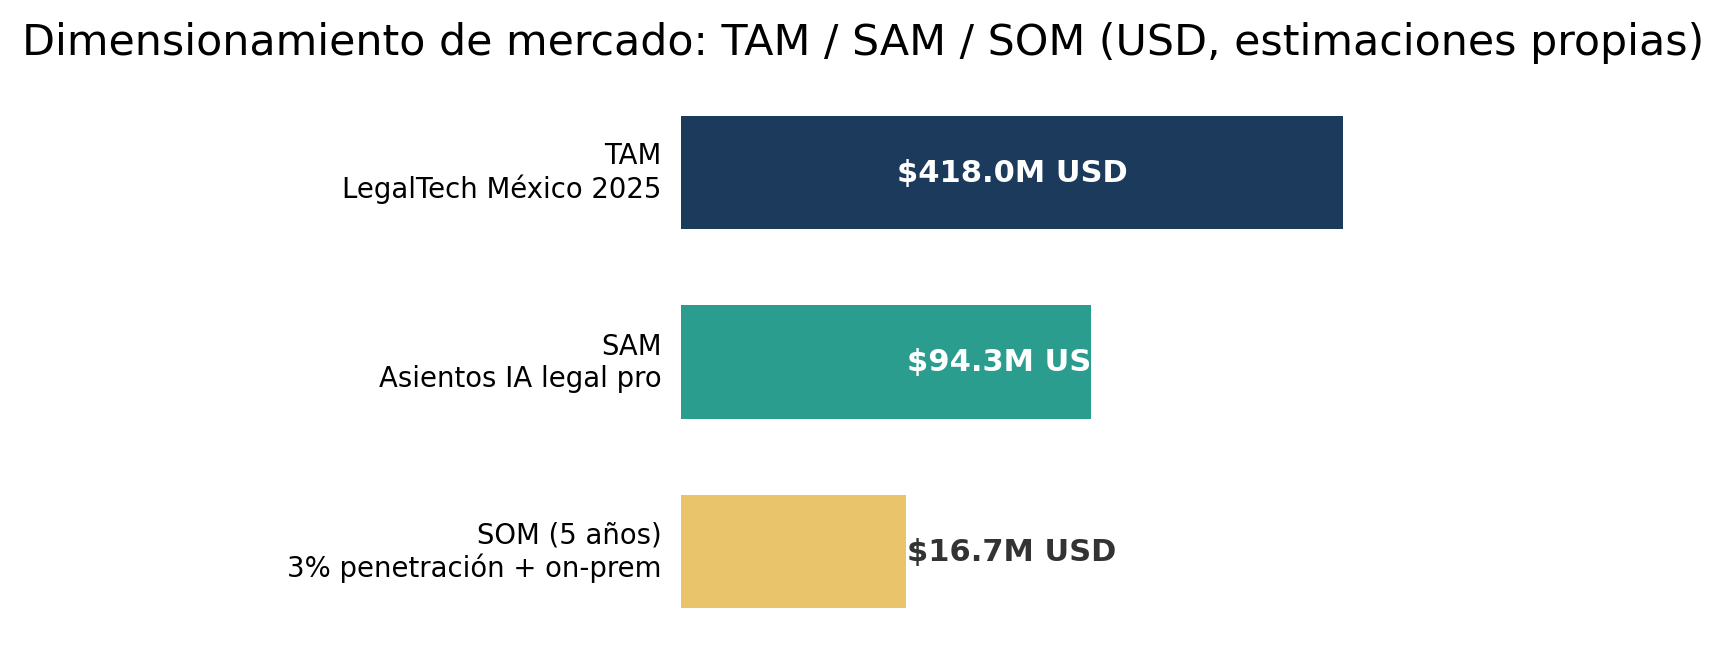
\includegraphics[width=0.84\textwidth]{fig_tam.png}
\caption{Dimensionamiento de mercado propio. TAM: 22\% del mercado LegalTech LatAm\cite{imarc2025}. SAM: asientos profesionales a USD 35/mes sobre la población abogacil\cite{mirada360,industryresearch2026} (precio de referencia incumbente: USD 300--500/mes\cite{vaquill2026}). SOM: penetración 3\% en asientos + 2\% de firmas en tier soberano.}
\label{fig:tam}
\end{figure}

\subsection{El efecto demostración: Harvey y la verticalización de la IA}

La viabilidad económica de la IA legal vertical ya no es hipotética. Harvey ---fundada en 2022--- alcanzó una valoración de \textbf{USD 11 mil millones} en marzo de 2026, con más de USD 1,000M levantados, $\sim$USD 190M de ARR a enero de 2026 ($\sim$USD 350M a mediados de año), 100,000+ abogados en 1,300 organizaciones y 60+ países;\cite{harvey2026,sacra2026} en agosto de 2026 negociaba una nueva ronda a USD 15.5 mil millones.\cite{theinformation2026} Legora levantó USD 550M a una valoración de USD 5.6 mil millones, y Thomson Reuters adquirió Casetext (CoCounsel) por USD 650M e invierte más de USD 200M anuales en IA.\cite{sacra2026,vlex2018,mordor2026} vLex (hoy parte de Clio) opera Vincent AI con cobertura anunciada para México entre otros 9+ países, sobre una biblioteca de 100M+ documentos.\cite{vlex2018,vlex2024}

Tres lecciones se desprenden para AI Justicia. Primera: el mercado premia la verticalización jurídica con múltiplos de frontera. Segunda: ninguno de estos actores compite en el segmento que ocupamos ---español mexicano, fuentes primarias locales, despliegue soberano, precio para la long tail de la abogacía; vLex, el más cercano en idioma, es SaaS en nube y no publica evaluación independiente de precisión.\cite{vaquill2026} Tercera: el análisis de la industria advierte que los modelos de frontera \emph{comoditizan} el razonamiento legal genérico, por lo que el valor migra a datos propietarios, orquestación de flujo y distribución.\cite{sacra2026} Eso es exactamente lo que un corpus vivo de 10B tokens de fuentes primarias mexicanas ---con un registro de cosecha diferencial que ningún competidor ha construido--- representa: \textbf{el activo no comoditizable}.

% ================= 3. MARCO REGULATORIO =================
\section{El marco regulatorio: por qué la soberanía es un requisito, no una opción}\label{sec:marco}

\subsection{La nueva LFPDPPP (2025) y el tratamiento automatizado}

El 20 de marzo de 2025 se publicó en el DOF la nueva Ley Federal de Protección de Datos Personales en Posesión de los Particulares, que abrogó la ley de 2010 y entró en vigor al día siguiente.\cite{lfpdppp} El cambio institucional más visible es la extinción del INAI ---por la reforma constitucional de simplificación orgánica de diciembre de 2024--- y la transferencia de sus atribuciones sobre datos del sector privado a la \textbf{Secretaría Anticorrupción y Buen Gobierno (SABG)}.\cite{ccn2025,lfpdppp} Las multas alcanzan \textbf{320,000 UMA} ($\sim\$37.5$ millones de pesos) y pueden duplicarse para datos personales sensibles.\cite{kyc2026}

Tres innovaciones de la ley son directamente relevantes para un sistema de IA jurídica. Primera, la ampliación de la definición de responsable: cualquier persona que realice tratamiento de datos tiene obligaciones directas, lo que captura a encargados y proveedores tecnológicos.\cite{cosio2026} Segunda, la eliminación de los ``fines análogos'': el responsable ya no puede tratar datos para finalidades distintas de las declaradas en el aviso de privacidad, aunque sean compatibles.\cite{ccn2025} Tercera ---y central---, las disposiciones sobre \textbf{tratamiento automatizado}: quien opere decisiones o tratamientos automatizados debe informar su existencia, explicar la lógica general del tratamiento y sus consecuencias posibles, y garantizar el derecho del titular a oponerse cuando produzcan efectos jurídicos adversos.\cite{cosio2026} Un asistente jurídico conversacional es, por definición, un tratamiento automatizado: su arquitectura de consentimiento, abstención y explicabilidad debe diseñarse alrededor de estos artículos, no como añadido cosmético. Al cierre de esta edición el reglamento de la ley seguía pendiente, lo que añade incertidumbre operativa pero no suspende las obligaciones vigentes.\cite{cosio2026}

\subsection{Secreto profesional con sanción penal}

El deber de sigilo del abogado no es solo deontológico. El Código Penal Federal sanciona la revelación de secretos o comunicaciones reservadas conocidas con motivo del empleo, cargo o puesto (art.~210, treinta a doscientas jornadas de trabajo comunitario) y la agrava cuando el revelador presta servicios profesionales o técnicos (art.~211, uno a cinco años, multa y suspensión de profesión de dos meses a un año).\cite{cpf} Enviar el expediente de un cliente a una API extranjera sin garantías contractuales y técnicas de no retención es una exposición penal y de responsabilidad civil que ningún comité de riesgos de despacho puede aceptar de forma permanente. La arquitectura de AI Justicia invierte la carga de la prueba: en el tier de despacho, \textbf{ningún dato sale del perímetro del cliente} ---modelo soberano on-premise, adaptadores LoRA privados, cero llamadas externas--- y el invariante de doble adaptador (Sección~\ref{sec:entrenamiento}) es la expresión arquitectónica de estos artículos.

\subsection{Base normativa del corpus: los textos del Estado no son objeto de derecho de autor}

La viabilidad legal del corpus descansa sobre una regla clara: el art.~14, fracc.~VII de la Ley Federal del Derecho de Autor establece que \textbf{no son objeto de protección} ``los textos legislativos, reglamentarios, administrativos o judiciales, así como sus traducciones oficiales'', añadiendo que su publicación deberá apegarse al texto oficial y no confiere derecho exclusivo de edición.\cite{lfda} Legislación federal y estatal, gacetas oficiales y sentencias judiciales son, por tanto, reutilizables para entrenamiento sin licencia autoral. La doctrina universitaria sigue reglas distintas: las fuentes incorporadas provienen de repositorios institucionales de acceso abierto (IIJ-UNAM vía OAI-PMH, repositorio de tesis UNAM), cuyos términos permiten consulta y reutilización académica; la redistribución del corpus sigue los términos de acceso público de cada fuente, todas ellas gubernamentales o universitarias de acceso abierto.

\subsection{Infraestructura: residencia de datos resuelta, soberanía de inferencia pendiente}

México vive una transformación de infraestructura cloud sin precedente: AWS invirtió más de USD 5,000M en su región de Querétaro (lanzada en 2025)\cite{aws2024} y Google Cloud inauguró la suya en diciembre de 2024, con latencias menores a 5 ms para el centro del país y una contribución estimada de USD 11,000M al PIB.\cite{gcp2024} Esto resuelve la \emph{residencia} del dato ---relevante para los tiers ciudadano y profesional--- pero no sustituye la soberanía de inferencia: el servicio gestionado de un hiperescalador extranjero sigue sujeto a políticas de retención, revisión y jurisdicción ajenas. La taxonomía de soberanía de IA aplicada en la literatura distingue corpus, entrenamiento, capacidad lingüística e inferencia;\cite{alia2026} AI Justicia cubre las cuatro: corpus nacional (Sección~\ref{sec:corpus}), entrenamiento propio sobre pesos abiertos (Sección~\ref{sec:entrenamiento}), capacidad jurídica en español mexicano, e inferencia dentro del perímetro del cliente en el tier de despacho.

% ================= 4. TRABAJO RELACIONADO =================
\section{Trabajo relacionado}\label{sec:relacionado}

\subsection{Modelos de lenguaje jurídicos: de SaulLM a la generación industrial}

SaulLM-7B (Colombo et al., Equall.ai, 2024) fue el primer LLM diseñado explícitamente para el dominio jurídico y sigue siendo la receta de referencia para el CPT de dominio.\cite{colombo2024} Construido sobre Mistral-7B, destila \textbf{30B tokens} de texto jurídico inglés a partir de \textbf{94B tokens crudos} ---descartando 68\% del material recolectado por artefactos de PDF, duplicados entre fuentes y unicode corrupto---, con fuentes que incluyen MultiLegal Pile, FreeLaw, GovInfo, EuroParl, EDGAR y USPTO. Sus dos decisiones metodológicas más influyentes son el \textbf{2\% de replay general} (Wikipedia, StackExchange, GitHub de SlimPajama) contra el olvido catastrófico, y la inclusión de \textbf{datos instruccionales durante el propio CPT} (FLAN, Super-NaturalInstructions) en lugar de diferir todo lo conversacional al SFT. El modelo se liberó bajo licencia MIT, y su escalado posterior a SaulLM-54B y SaulLM-141B documentó los trade-offs de la adaptación de dominio a mayor escala.\cite{saullm54b} La lección que importa: \emph{la ingeniería de calidad del corpus domina al volumen}.

En el plano industrial, la generación de modelos legales propietarios de la familia de Thomson Reuters ---referenciada en nuestro borrador de trabajo como Thomson-1.0, cuyo reporte técnico (2025) describe un MoE de clase 35B sobre la misma familia base que empleamos--- validó dos decisiones que adoptamos: \textbf{CPT fuerte más fusión lineal de modelos} como mecanismo anti-olvido (en lugar de replay solo), y un currículo multietapa sobre corpus jurídicos propietarios de decenas de miles de millones de tokens. Su licencia (PolyForm Strict, no comercial) impide usar el modelo, pero sus \emph{decisiones de arquitectura} son reproducibles; nuestra evaluación empírica (Sección~\ref{sec:problema}) confirmó tanto su lección principal como su límite: el modelo produce respuestas con \emph{forma de abogado} pero sigue alucinando números de artículo específicos de jurisdicción.

\subsection{LLMs jurídicos fuera del mundo anglosajón}

La literatura confirma que la verticalización jurisdiccional es viable y útil fuera del inglés. China ha producido una familia completa de LLMs legales ---ChatLaw (multiagente, con base de conocimiento externa y módulo de referencia explícitamente diseñado para reducir alucinación),\cite{cui2024chatlaw} DISC-LawLLM, Fuzi-Mingcha, HanFei, InternLM2-Law y LawGPT--- entrenados sobre legislación, interpretaciones judiciales y foros legales chinos.\cite{surveylegal2025} Para el español, los recursos a escala existentes (Legal-ES; la tarea compartida IberLegal de IberLEF) se concentran en NER sobre textos jurídicos y administrativos \emph{de España}.\cite{legales2020} En el plano de modelos soberanos nacionales, el proyecto español Alia ---impulsado por el gobierno con corpus curados y supervisión pública--- ejemplifica la motivación de soberanía lingüística, aunque sus propios analistas reconocen que no resuelve la capa que más importa a los sectores regulados: la soberanía de inferencia.\cite{alia2026} \textbf{Para el derecho mexicano no existe, a la fecha, ningún corpus de entrenamiento a escala ni ningún modelo de dominio publicado.} Ese vacío es simultáneamente la motivación científica y la oportunidad de negocio de este proyecto.

\subsection{La medición de la alucinación legal}

El estado del arte empírico se resume en tres resultados. (i) Dahl et al.: alucinación del 58--88\% en modelos generales, con degradación en jurisdicciones poco prominentes y ausencia de autoconciencia del error.\cite{dahl2024} (ii) Magesh et al.: las herramientas RAG comerciales reducen pero no eliminan el problema (17--33\%), y el modo residual más peligroso es la cita \emph{misgrounded} ---fuente real que no sustenta la afirmación---, indistinguible sin leer la fuente.\cite{magesh2025} (iii) El ensayo controlado de Schwarcz et al. con estudiantes de derecho: el RAG preserva la integridad factual de no usar IA; el modelo de razonamiento sin anclaje mejora el análisis pero contamina con alucinaciones.\cite{ailawlibrarians2026} La conclusión de ingeniería es estable: \textbf{la fiabilidad legal exige anclaje en recuperación en inferencia}, y la pregunta abierta ---que abordamos--- es si ese comportamiento de anclaje puede además \emph{entrenarse en los pesos}.

\begin{table}[H]
\centering\small
\caption{Síntesis comparativa del trabajo relacionado y posición de AI Justicia.}
\label{tab:relacionado}
\begin{tabular}{@{}p{3.1cm}p{2.6cm}p{3.0cm}p{2.6cm}p{2.6cm}@{}}
\toprule
\textbf{Sistema} & \textbf{Jurisdicción / idioma} & \textbf{Corpus} & \textbf{Anclaje factual} & \textbf{Despliegue soberano} \\
\midrule
SaulLM-7B\cite{colombo2024} & Anglosajón / inglés & 30B tokens (abierto, MIT) & No (bare) & Sí (pesos abiertos) \\
SaulLM-54B/141B\cite{saullm54b} & Anglosajón / inglés & Escalado, MIT & No (bare) & Sí \\
ChatLaw et al.\cite{cui2024chatlaw,surveylegal2025} & China / chino & Corpus legal chino & KB + referencia & Parcial \\
Legal-ES / IberLegal\cite{legales2020} & España / español & Recursos NER & N/A (tarea) & Sí (recursos) \\
Lexis+ AI / Westlaw AI\cite{magesh2025} & EE.UU. / inglés & Propietario & RAG (17--33\% aluc.) & No (SaaS) \\
vLex Vincent\cite{vlex2024} & 9+ países incl. México & 100M+ docs & RAG (no evaluado indep.) & No (SaaS) \\
Harvey\cite{harvey2026} & Global / inglés-céntrico & Propietario & RAG + workflows & No (SaaS) \\
\midrule
\textbf{AI Justicia} & \textbf{México / español} & \textbf{10B+ tokens vivos} & \textbf{RAG + harness training + abstención} & \textbf{Sí (on-premise)} \\
\bottomrule
\end{tabular}
\end{table}

% ================= 5. EL CORPUS =================
\section{El corpus: 10B tokens de derecho mexicano}\label{sec:corpus}

\subsection{Composición}

El corpus de AI Justicia se construye exclusivamente sobre fuentes primarias mexicanas ---legislación, gacetas, jurisprudencia y doctrina--- más un conjunto instructivo en inglés restringido al SFT. La Tabla~\ref{tab:corpus} y la Figura~\ref{fig:corpus} resumen su composición. El estado actual es de \textbf{más de 1.5B tokens ingeridos y consultables}, con el resto en cosecha activa y un universo descubierto y accesible superior a 12B tokens.

\begin{table}[H]
\centering\small
\caption{Composición del corpus AI Justicia por familia de fuentes.}
\label{tab:corpus}
\begin{tabular}{@{}p{4.6cm}p{6.4cm}r@{}}
\toprule
\textbf{Familia} & \textbf{Contenido} & \textbf{Tokens aprox.} \\
\midrule
Semanario Judicial de la Federación\cite{sjf} & 150K jurisprudencias y tesis aisladas & $\sim$22M \\
DOF federal\cite{sidof} & 1999--2026, texto completo por nota & $\sim$300M+ \\
Legislación federal y reglamentos & Corpus LeyesBiblio, reglamentos, manuales & $\sim$38M \\
Legislación estatal (32 estados) & Códigos, leyes y reglamentos consolidados & $\sim$85M \\
Gaceta CDMX & Archivo completo 2014--2026 (vía Wayback CDX) & 143M \\
Caselaw CDMX (SIVEPJ) & 28,146 sentencias, universo completo enumerado & $\sim$34M \\
Caselaw Edomex & $\sim$85K sentencias públicas únicas (API judicial) & $\sim$3--4B \\
Caselaw Jalisco & 84,371 sentencias vía URLs firmadas S3 & $\sim$2--3B \\
Caselaw Querétaro, NL y otros & Cadenas JWT, cosecha ASP.NET & $\sim$1--2B \\
Doctrina: BJV (IIJ-UNAM) & 5,680 libros completos vía OAI-PMH & $\sim$1B \\
Tesis: Repositorio UNAM & 43,423 tesis ($\sim$40\% con PDF completo) & $\sim$2--3B \\
Instructivo inglés (solo SFT) & 269K ejemplos de razonamiento: NLI contractual, lógica LSAT, case briefs; \textbf{cero legislación extranjera} & mezcla SFT \\
\bottomrule
\end{tabular}
\end{table}

\begin{figure}[H]
\centering
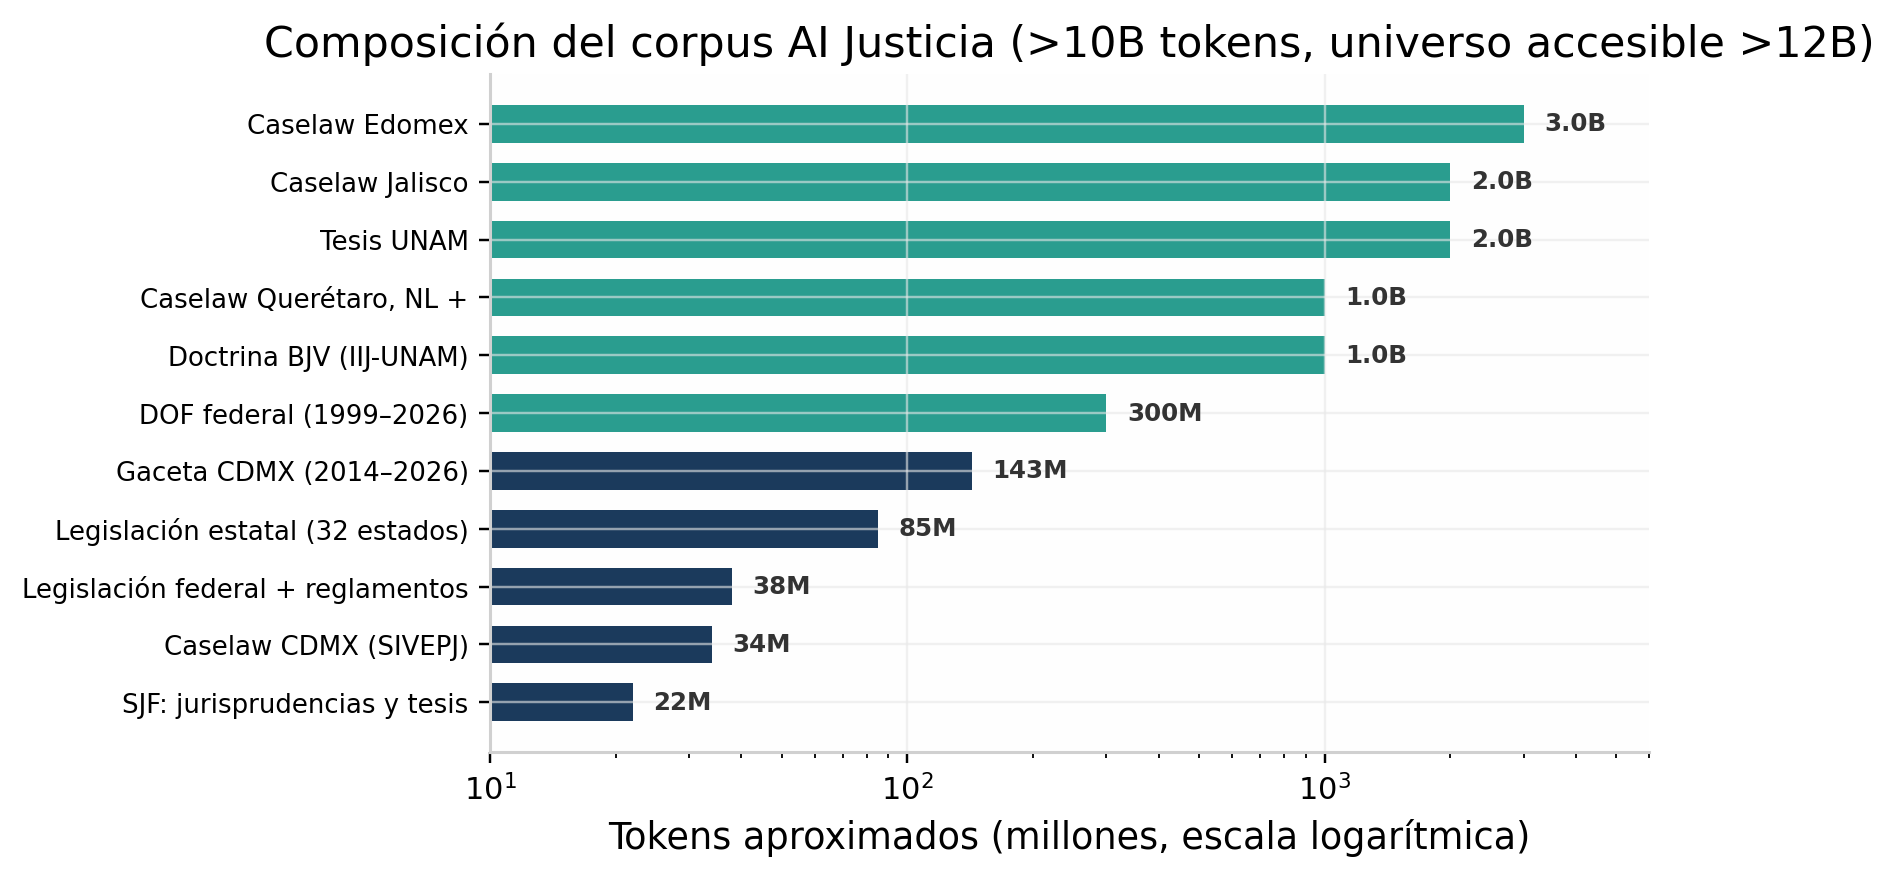
\includegraphics[width=0.95\textwidth]{fig_corpus.png}
\caption{Composición del corpus por familia de fuentes (escala logarítmica). El derecho anglosajón de SaulLM fue 30B tokens de una jurisdicción consolidada;\cite{colombo2024} el corpus mexicano alcanza escala comparable en orden de magnitud pero desde 33+ jurisdicciones internas heterogéneas.}
\label{fig:corpus}
\end{figure}

\subsection{Ingeniería de datos: la parte reproducible que nadie publica}

Cada fuente exigió ingeniería inversa a medida. Documentamos las técnicas porque son el verdadero cuello de botella de la IA jurídica en la mayoría de los países ---y, en consecuencia, el activo más difícil de replicar del proyecto:

\begin{itemize}
\item \textbf{OAI-PMH donde existe} (IIJ-UNAM): el camino limpio ---tokens de resumición y re-cosecha incremental por \emph{datestamp}.
\item \textbf{APIs Elasticsearch abiertas} (judicatura Edomex): el límite de 10K por slice obliga a sub-dividir por trimestre; los PDF se sirven desde un host de archivos predecible separado.
\item \textbf{APIs tras reCAPTCHA} (STJ Jalisco): la cookie de sesión \texttt{\_vt} está ligada a IP y tiene cuota; sostenemos la cosecha manejando un navegador real vía CDP, renovando la cookie con recargas completas (que re-ejecutan \texttt{grecaptcha} con score aceptable) y consultando el listado por \texttt{curl} con la cookie extraída, mientras los PDF provienen de URLs pre-firmadas de S3 que no requieren sesión.
\item \textbf{Portales con cadenas JWT} (Querétaro): el endpoint de lista devuelve llaves estructuradas $\rightarrow$ endpoint de token por documento (TTL 60s) $\rightarrow$ endpoint de PDF. HTTP puro, sin navegador.
\item \textbf{Portales geo-bloqueados} (Consejería Jurídica CDMX, SEGOB Veracruz): cosecha desde una máquina con IP mexicana y envío de JSONL al servidor de datos.
\item \textbf{Wayback CDX como rescate de archivo legal}: el buscador propio de la gaceta CDMX es una aplicación ZK Java inautomatizable; el archivo completo de PDF existe en el índice de la Wayback Machine y es totalmente enumerable.
\item \textbf{Doctrina escaneada $\rightarrow$ OCR}: Apple Vision OCR (es-ES, $\sim$0.7 s/página) recuperó 445 cuadernillos de la SCJN y libros doctrinales completos sin texto embebido.
\item \textbf{Todo diferencial}: el script, estado de marca de agua y estrategia incremental de cada cosechador vive en un registro PostgreSQL (\texttt{harvest\_scripts}). Las leyes cambian, las gacetas publican a diario, los tribunales suben constantemente: un corpus de derecho mexicano no es un dataset; es un \textbf{sistema vivo de registro} ---actualmente 17 fuentes registradas.
\end{itemize}

Esta capa de ingeniería es también la respuesta a la pregunta de defensibilidad: un competidor con capital puede rentar GPUs en una tarde (Sección~\ref{sec:viabilidad}), pero no puede reconstituir años de cosecha diferencial, normalización y verificación sobre 33+ portales heterogénicos sin repetir el mismo trabajo.

% ================= 6. ESTRATEGIA DE ENTRENAMIENTO =================
\section{Arquitectura del sistema y estrategia de entrenamiento}\label{sec:entrenamiento}

\subsection{El sistema en producción}

AI Justicia es un sistema en producción (\url{https://aijusticia.mx}) con tres tiers de servicio: \textbf{ciudadano} (gratuito, anónimo, guiado por entrevista), \textbf{abogado} (modo profesional, registro técnico, generación de documentos) y \textbf{despacho} (modelo soberano on-premise con adaptadores privados). Toda consulta atraviesa el mismo pipeline:

\begin{enumerate}
\item \textbf{Análisis} --- clasificación de materia y detección de jurisdicción (federal vs. 32 estados).
\item \textbf{Normalización} --- lenguaje ciudadano coloquial $\rightarrow$ terminología estatutaria (``me despidieron'' $\rightarrow$ ``despido injustificado \dots{} art.~48 LFT''). Esta etapa mejoró drásticamente la recuperación FTS.
\item \textbf{Entrevista} --- rondas dinámicas de clarificación manejadas por el LLM (configurables pre/post-recuperación) que construyen un expediente estructurado.
\item \textbf{Recuperación} --- búsqueda de texto completo PostgreSQL con stemming en español sobre el corpus, ponderada por fuente (estatutos 1.3$\times$, jurisprudencia 1.2$\times$), con filtrado de relevancia.
\item \textbf{Generación} --- respuestas ancladas: toda afirmación jurídica debe portar una cita \texttt{[n]} a un pasaje recuperado.
\item \textbf{Verificación} --- pasada de \emph{entailment} sobre cada oración citada; bajo el umbral de soporte, el sistema \textbf{abstiene honestamente} en lugar de responder.
\end{enumerate}

\paragraph{La lección de la abstención.} Nuestra primera evaluación completa mostró 93\% de abstención: el sistema rechazaba casi todo. La causa raíz no era el modelo sino \emph{cómo lo llamábamos}: el modelo de razonamiento empleado consume 5--8K tokens de pensamiento interno antes de responder; nuestros presupuestos por etapa (128--256 tokens para normalización y filtrado) truncaban el pensamiento a la mitad, produciendo salidas vacías $\rightarrow$ consultas coloquiales llegaban al FTS $\rightarrow$ pasajes irrelevantes $\rightarrow$ abstención. Tras corregir presupuestos (10K mínimo) y añadir una segunda pasada autocorrectiva para formatos de cita débiles, la tasa de respuesta pasó de \textbf{2/30 a 18/30} sin pérdida de integridad de citas. Lección: para modelos de razonamiento, la ingeniería de prompts incluye \emph{ingeniería de presupuesto de tokens}.

\subsection{La receta de entrenamiento de Tlamatini}

Tlamatini (náhuatl: el que sabe cosas'') es el nombre del modelo soberano. La virtud epistémica que lo define es la que su nombre evoca: el sabio aconseja y, crucialmente, admite lo que no sabe ---nuestra abstención honesta. La infraestructura de entrenamiento lleva el nombre de \emph{Tohil} (el fuego que forja: los runs de CPT en GPU rentada).

Sintetizando SaulLM, la generación industrial y nuestros hallazgos de evaluación:

\begin{enumerate}
\item \textbf{Base}: la misma familia del modelo industrial de referencia (MoE clase 35B con $\sim$3B parámetros activos) ---decisión de arquitectura ya validada por ese reporte y verificable en nuestra máquina de desarrollo local, que corre la arquitectura en cuantización de 4 bits. Una alternativa densa de la generación más reciente (27B, Apache 2.0, contexto 256K) está en evaluación: el MoE abarata CPT ($\sim$6$\times$ en cómputo activo) e inferencia on-premise, pero el CPT sobre modelos densos es más estable (el \emph{routing drift} de MoE es un riesgo conocido); la decisión se toma con la misma batería de 30 preguntas descrita en \S
ef{sec:problema}.
\item \textbf{Etapa 1 --- CPT full-parameter} sobre el corpus mexicano ($\sim$10B tokens): $\sim$80\% derecho primario mexicano en su mezcla natural (siguiendo a SaulLM: deduplicación agresiva, sin sobreponderación artificial de estatutos sobre caselaw\cite{colombo2024}); $\sim$15\% ejemplos en formato harness (\S\ref{sec:harness}); $\sim$2--5\% replay general (Wikipedia en español, código, instructivo general). Full-parameter y no LoRA-CPT: nuestro intento previo de LoRA-CPT a LR alta divergió (val loss $1.24 \rightarrow 10.69$), y el análisis de costos (Figura~\ref{fig:costo}) hace innecesario el atajo. \textbf{Fusión lineal con el modelo base} post-CPT como mecanismo anti-olvido.
\item \textbf{Etapa 2 --- SFT} sobre: diálogo guiado por entrevista, respuestas ancladas en citas, calibración de abstención; más los 269K ejemplos instructivos ingleses de razonamiento (NLI contractual, lógica tipo LSAT, case briefs ---patrones de razonamiento, cero estatutos extranjeros).
\item \textbf{Etapa 3 --- adaptadores por despacho}: adaptadores LoRA privados entrenados exclusivamente sobre documentos consentidos de cada firma, servidos por fusión en runtime. \textbf{El invariante de doble adaptador}: los datos de un despacho jamás entran al adaptador general; el adaptador general jamás ve documentos privilegiados. Es la expresión arquitectónica de los arts.~210--211 CPF y de la LFPDPPP.\cite{cpf,lfpdppp}
\end{enumerate}

\subsection{Harness training: enseñar el harness en los pesos}\label{sec:harness}

Nuestro sistema de producción es un harness: recuperar pasajes $\rightarrow$ inyectarlos como contexto $\rightarrow$ exigir respuestas ancladas en citas. Todos nuestros fallos de abstención fueron fallos de harness (formato perdido, presupuesto de pensamiento agotado). La extensión natural ---propuesta independientemente en la literatura reciente como \emph{harness training}--- es \textbf{entrenar el comportamiento del harness en el propio modelo}, incluyendo millones de ejemplos en el formato exacto de inferencia durante el CPT:

\begin{center}
\ttfamily\small
<pasaje(s) recuperado(s)> + <pregunta ciudadana> $\rightarrow$ <respuesta con anclas [n] por afirmación>
\end{center}

Tres fuentes de pares harness, todas ya en mano: (i) \textbf{el propio caselaw}: los considerandos judiciales son naturalmente aserción-más-artículo ---minar pares (considerando $\rightarrow$ artículo citado) de las 200K+ sentencias produce datos en formato anclado gratis; (ii) \textbf{trazas de producción}: con consentimiento ciudadano explícito y revocable conforme a LFPDPPP, nuestros logs verificados de consulta$\rightarrow$pasajes$\rightarrow$respuesta son oro de la distribución real del harness; (iii) \textbf{destilación sintética}: pasaje $\rightarrow$ generar pregunta ciudadana + respuesta anclada, a escala de corpus.

\begin{tesis}
\textbf{Aportación central.} El CPT de dominio produce la \emph{forma} correcta de la respuesta (Thomson); la recuperación produce los \emph{hechos} correctos (nuestra evaluación RAG); el harness training los unifica. Para IA jurídica jurisdicción-específica, \emph{harness-en-los-pesos} + \emph{recuperación-en-inferencia} supera a cada estrategia por separado.
\end{tesis}

\subsection{Qué mediremos}

\begin{itemize}
\item Batería ciudadana de 30 preguntas: tasa de respuesta, precisión de cita, exactitud a nivel de artículo ---el modo de falla que exhibieron las respuestas bare del modelo industrial.
\item QA estatutario con sensibilidad a reformas (misma pregunta, año pre/post reforma).
\item Calibración de abstención: tasa de falsa abstención vs. tasa de alucinación.
\item Modo profesional: redacción de promociones y contratos evaluada por abogados en ejercicio.
\end{itemize}

% ================= 7. VIABILIDAD DE NEGOCIO =================
\section{Viabilidad de negocio}\label{sec:viabilidad}

\subsection{Modelo de ingresos por tiers}

El diseño de tres tiers no es solo de producto: es una secuencia de adquisición. El tier ciudadano (gratuito, anónimo, sin email ---recuperación por frase, datos locales hasta opt-in explícito) ataca el déficit de acceso y genera la distribución; el tier abogado (suscripción a fracción del precio incumbente) monetiza el uso profesional; el tier despacho (licencia anual on-premise con adaptadores privados) captura el segmento donde el cumplimiento es innegociable y el precio es secundario.

\begin{table}[H]
\centering\small
\caption{Tiers de producto, precios objetivo y justificación de mercado.}
\label{tab:tiers}
\begin{tabular}{@{}p{2.2cm}p{4.6cm}p{3.4cm}p{3.8cm}@{}}
\toprule
\textbf{Tier} & \textbf{Propuesta} & \textbf{Precio objetivo} & \textbf{Referencia de mercado} \\
\midrule
Ciudadano & Entrevista guiada, orientación anclada, abstención honesta & Gratuito (adquisición) & 32M problemas jurídicos/año; 70\% no busca asesoría\cite{wjpmx2019} \\
Abogado & Modo profesional, documentos, corpus completo & USD $\sim$35/asiento/mes & Incumbentes: USD 300--500/mes\cite{vaquill2026}; salario promedio abogado MX $\sim\$13.3$k MXN\cite{forojuridico2023} \\
Despacho & Modelo soberano on-premise, adaptadores LoRA privados, cero llamadas externas & USD $\sim$12,000/año & On-premise conserva $\sim$63\% del despliegue LegalTech por control de información\cite{fortune2026} \\
Corpus & Licenciamiento del registro de cosecha y corpus curado a instituciones & Por acuerdo & No existe equivalente mexicano (Sección~\ref{sec:corpus}) \\
\bottomrule
\end{tabular}
\end{table}

\subsection{Unit economics: el cómputo no es el problema}

El costo de entrenar el modelo base soberano es sorprendentemente bajo. Con la regla estándar de $6ND$ FLOPs\cite{spheron} aplicada a un MoE de $\sim$3B parámetros activos sobre 10B tokens, el run principal de CPT requiere $\sim 1.8\times10^{20}$ FLOPs: entre \textbf{100 y 170 GPU-horas} de clase H100/H200 según la eficiencia (MFU 30--50\%), es decir, del orden de \textbf{USD 260--1,000} a precios de mercado spot (\$2.6/GPU-h) o USD 600--1,000 a tarifas on-demand altas (\$6/GPU-h)\cite{gmicloud2026,introl2026} ---menos de dos días de reloj en 4$\times$H200. Incluso con diez runs de experimentación, ablación y fallos, el presupuesto total de cómputo de entrenamiento queda en los miles de dólares, no en los millones. Los costos de inferencia son igualmente manejables: servir un modelo 70B-cuántizado en H200 cuesta $\sim$USD 5/1M tokens,\cite{gmicloud2026} y la cuantización INT4 reduce 75\% el costo por token con 1--2\% de degradación.\cite{introl2026}

\begin{figure}[H]
\centering
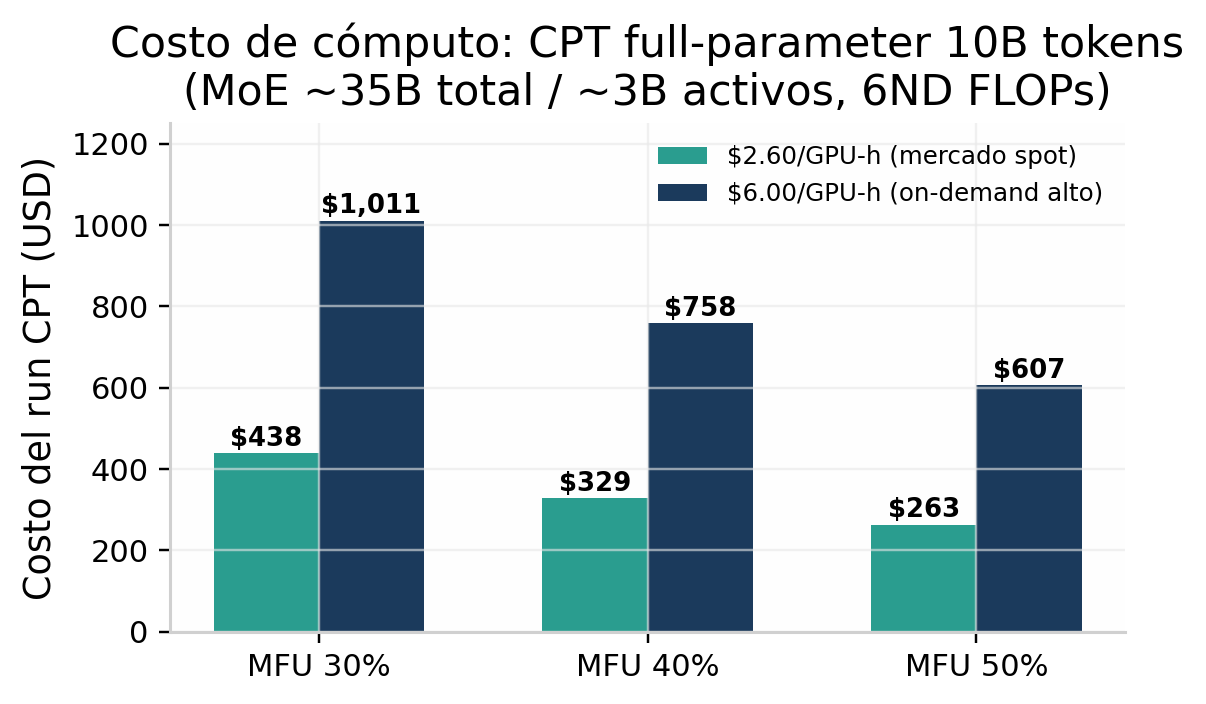
\includegraphics[width=0.82\textwidth]{fig_costo_cpt.png}
\caption{Costo estimado del run principal de CPT (10B tokens, MoE $\sim$3B activos, regla $6ND$; precios GPU de mercado\cite{gmicloud2026,introl2026,spheron}). El cómputo es marginal; el activo escaso es el corpus.}
\label{fig:costo}
\end{figure}

La conclusión económica invierte la intuición habitual: \textbf{la barrera no es el capital de cómputo sino la ingeniería de datos acumulada}. Esto tiene una implicación de estrategia competitiva directa: el proyecto debe defender y capitalizar el corpus (registro diferencial, normalización, licenciamiento) más que el modelo, porque los pesos son recomputables por cualquiera con el mismo corpus ---y nadie más lo tiene.

\subsection{Posición competitiva}

La Tabla~\ref{tab:relacionado} resume el panorama: los incumbentes globales (Harvey, CoCounsel/Westlaw, Lexis+, vLex) compiten en SaaS anglocéntrico de USD 300--500/asiento/mes;\cite{vaquill2026} las legaltech mexicanas (25+ startups) compiten en gestión y automatización sin modelos propios;\cite{computerweekly2025} y los modelos abiertos legales (SaulLM) no cubren jurisdicción ni español mexicano.\cite{colombo2024} La posición de AI Justicia ---español mexicano, corpus primario vivo, anclaje con abstención, on-premise, precio long tail--- no solapa frontalmente con ninguno. El riesgo de commoditización que los analistas identifican para la IA legal vertical (los modelos de frontera igualan el razonamiento genérico)\cite{sacra2026} refuerza, no debilita, esta tesis: lo que no se comoditiza son los datos jurisdiccionales y el cumplimiento.

El español como plataforma de expansión es un upside no contado en el SOM: con 520M de hablantes nativos y 635M potenciales ---tercera comunidad lingüística del mundo---,\cite{cervantes2025} la misma metodología (cosecha diferencial + harness training) es replicable en otras jurisdicciones de tradición civil hispanohablante, donde el vacío de corpus es idéntico al mexicano.

\subsection{Escenarios financieros a 5 años}

\begin{table}[H]
\centering\small
\caption{Escenarios de ARR a 5 años (estimaciones propias sobre los parámetros de la Sección~\ref{sec:necesidad}).}
\label{tab:escenarios}
\begin{tabular}{@{}lrrr@{}}
\toprule
\textbf{Línea} & \textbf{Conservador} & \textbf{Base} & \textbf{Optimista} \\
\midrule
Asientos abogado (1\% / 3\% / 5\% de 449K) & \$1.9M & \$5.7M & \$9.4M \\
Despachos on-premise (0.5\% / 2\% / 4\% de 46K) & \$2.8M & \$11.0M & \$22.1M \\
Corpus e instituciones & \$0.2M & \$0.8M & \$2.0M \\
\midrule
\textbf{ARR total} & \textbf{\$4.9M} & \textbf{\$17.5M} & \textbf{\$33.5M} \\
\bottomrule
\end{tabular}
\end{table}

Los supuestos son deliberadamente sobrios: penetraciones de un dígito sobre poblaciones medidas (449K abogados, 46K firmas),\cite{mirada360,industryresearch2026} precios una décima parte del incumbente,\cite{vaquill2026} y ningún ingreso del tier ciudadano. El costo marginal del cómputo de entrenamiento e inferencia (Figura~\ref{fig:costo}) permite sostener márgenes de software incluso al precio long tail que el mercado mexicano exige.

% ================= 8. RIESGOS =================
\section{Riesgos y limitaciones}\label{sec:riesgos}

\begin{table}[H]
\centering\small
\caption{Registro de riesgos principales y mitigaciones.}
\label{tab:riesgos}
\begin{tabular}{@{}p{3.4cm}p{4.9cm}p{5.6cm}@{}}
\toprule
\textbf{Riesgo} & \textbf{Descripción} & \textbf{Mitigación} \\
\midrule
Alucinación residual & El RAG reduce pero no elimina el error (17--33\% en incumbentes\cite{magesh2025}); el modo \emph{misgrounded} es indetectable sin leer la fuente & Verificación por \emph{entailment} por oración + abstención honesta + evaluación continua; métricas públicas de la batería de 30 preguntas \\
Responsabilidad por consejo legal & Un ciudadano puede tomar la orientación como asesoría definitiva & Diseño de abstención, disclaimers estructurales, referencia a instituciones; el sistema orienta, no litiga; tratamiento automatizado declarado conforme a LFPDPPP\cite{cosio2026} \\
Incertidumbre regulatoria & El reglamento de la LFPDPPP 2025 sigue pendiente; la SABG es autoridad nueva\cite{cosio2026,kyc2026} & Cumplimiento por diseño (opt-in revocable, minimización, local-first); monitoreo regulatorio como parte del corpus vivo \\
Obsolescencia del corpus & Reformas legislativas y criterios nuevos degradan el anclaje & Cosecha diferencial con registro persistente (17 fuentes); sensibilidad a reformas como métrica de evaluación \\
Competencia de incumbentes & Harvey/vLex podrían localizar para México\cite{harvey2026,vlex2024} & El foso es el corpus vivo + on-premise + precio; replicar la cosecha diferencial toma años \\
Fragilidad de fuentes & Cambios en portales, reCAPTCHAs, términos de acceso & Registro de harvesters con estrategia por fuente; redundancia (Wayback CDX); OAI-PMH incremental donde existe \\
Base modelo abierto & Dependencia de familias de pesos abiertos (licencias, disponibilidad) & Arquitectura agnóstica de base; fusión lineal preserva reversibilidad al base \\
Sesgo de evaluación & La batería de 30 preguntas es propia y pequeña & Prerregistro de métricas, evaluación por abogados en ejercicio, publicación de metodología \\
\bottomrule
\end{tabular}
\end{table}

Dos limitaciones metodológicas merecen declararse explícitamente. Primera, las cifras de mercado provienen de firmas de análisis con metodologías heterogéneas (IMARC, Mordor, Fortune BI difieren en el tamaño absoluto del mercado global, aunque coinciden en rango y CAGR);\cite{imarc2025,mordor2026,fortune2026} nuestro TAM/SAM/SOM deriva de supuestos propios conservadores y debe leerse como orden de magnitud, no como proyección financiera auditada. Segunda, las métricas de desempeño del sistema (batería de 30 preguntas, tasas de abstención) son evaluaciones internas del proyecto, aún no auditadas por terceros; su publicación con metodología abierta es parte de la hoja de ruta.

% ================= 9. HOJA DE RUTA =================
\section{Estado actual y hoja de ruta}\label{sec:roadmap}

\begin{table}[H]
\centering\small
\caption{Estado y hitos del proyecto.}
\label{tab:roadmap}
\begin{tabular}{@{}p{2.6cm}p{5.2cm}p{5.8cm}@{}}
\toprule
\textbf{Frente} & \textbf{Estado (agosto 2026)} & \textbf{Siguiente hito} \\
\midrule
Corpus & 1.5B+ tokens ingeridos y consultables; 10B+ accesibles; 17 fuentes registradas & Completar cosecha de caselaw estatal (Edomex, Jalisco, Querétaro, NL); publicar ficha técnica del corpus \\
Sistema & Producción en aijusticia.mx (tiers ciudadano y abogado); harness con abstención; respuesta 2/30 $\rightarrow$ 18/30 tras corrección de presupuestos & Batería de evaluación automatizada y prerregistrada; modo profesional con evaluación por abogados \\
Modelo base & Arquitectura validada; receta fijada (CPT + merge + harness training); corrida CPT planificada en 4$\times$H200 rentadas (Figura~\ref{fig:costo}) & Run CPT sobre corpus completo; fusión lineal; SFT; liberación de resultados de evaluación \\
Tier despacho & En desarrollo, pendiente del modelo base & Primer piloto on-premise con adaptadores privados e invariante de doble adaptador \\
Cumplimiento & Opt-in ciudadano revocable; anonimato por diseño; avisos conforme a LFPDPPP 2025\cite{lfpdppp,cosio2026} & Actualización al reglamento de la LFPDPPP cuando se publique; auditoría de terceros \\
\bottomrule
\end{tabular}
\end{table}

\subsection{Contribuciones}

\begin{enumerate}
\item El primer \textbf{corpus vivo de derecho mexicano} a escala documentada (10B+ tokens), con registro de cosecha diferencial y técnicas reproducibles para cada fuente ---un activo de infraestructura de investigación por derecho propio.
\item Un \textbf{asistente jurídico anclado en recuperación} en producción, con abstención honesta, evaluado en tres configuraciones (generalista en nube +RAG vs. fundación legal +RAG vs. fundación legal bare), incluyendo la identificación y corrección de la patología de presupuesto de tokens de modelos de razonamiento en pipelines RAG.
\item Una \textbf{receta de entrenamiento} que unifica replay de SaulLM, fusión lineal industrial y harness training, orientada al primer modelo base legal soberano de México, con costo de cómputo de tres cifras en dólares.
\item Evidencia de que la \textbf{alucinación de citas sobrevive al CPT de dominio}: el anclaje jurisdiccional requiere recuperación, y el formato del harness puede entrenarse en los pesos.
\item Un \textbf{análisis de viabilidad} que documenta la necesidad social (32M de problemas jurídicos/año, 5\% de acceso institucional\cite{wjpmx2019,justiciaabierta2025}), el mercado (TAM $\sim$USD 418M, SOM USD 5--17M ARR) y la restricción regulatoria que hace de la soberanía un requisito de cumplimiento (LFPDPPP 2025; arts.~210--211 CPF).\cite{lfpdppp,cpf}
\end{enumerate}

% ================= 10. CONCLUSIONES =================
\section{Conclusiones}\label{sec:conclusiones}

La pregunta que originó este whitepaper ---si existe necesidad y viabilidad de negocio para un LLM jurídico mexicano local--- admite una respuesta afirmativa con evidencia en los tres planos analizados.

En el plano de la \textbf{necesidad}, el déficit está medido: la mitad de los mexicanos enfrenta problemas jurídicos cada dos años, solo 30\% busca asesoría y 5 de cada 100 alcanzan una institución;\cite{wjpmx2019,justiciaabierta2025} el poder judicial opera con rezago estructural y menos juzgadores;\cite{eleconomista2025} y los modelos disponibles alucinan el derecho mexicano con fluidez profesional, porque el anclaje jurisdiccional no se entrena ---se recupera, y hoy no hay de dónde recuperarlo.\cite{dahl2024,magesh2025}

En el plano de la \textbf{factibilidad técnica}, la receta existe y está validada por partes: SaulLM demostró que 30B tokens de dominio con replay producen un modelo legal utilizable bajo licencia abierta;\cite{colombo2024} la generación industrial demostró que CPT fuerte más fusión lineal escala a producción; la literatura de alucinación demostró que el RAG es indispensable pero insuficiente sin verificación y abstención;\cite{magesh2025,ailawlibrarians2026} y nuestro propio sistema demostró en producción que el harness anclado con abstención honesta es operable hoy. El costo de cómputo del modelo base ---cientos de dólares, no millones--- convierte la pregunta de factibilidad en una pregunta de datos, y los datos ya están siendo cosechados con base normativa sólida (art.~14-VII LFDA).\cite{lfda}

En el plano de la \textbf{viabilidad de negocio}, el mercado premia exactamente lo que el proyecto construye: la verticalización legal de la IA vale decenas de miles de millones en los mercados anglosajones (Harvey, Legora, CoCounsel);\cite{harvey2026,sacra2026} el mercado LegalTech latinoamericano crece a doble dígito;\cite{imarc2025} la abogacía mexicana es numerosa, atomizada y subdigitalizada;\cite{mirada360,computerweekly2025} y la regulación mexicana ---LFPDPPP 2025 con sus reglas de tratamiento automatizado, y el deber penal de sigilo--- convierte el despliegue soberano en la única opción jurídicamente defendible para el segmento de mayor valor: los despachos.\cite{lfpdppp,cosio2026,cpf} El foso defensivo no es el modelo, que es recomputable, sino el corpus vivo y el cumplimiento, que no lo son.

El trabajo inmediato es el que la hoja de ruta detalla: completar la cosecha de caselaw estatal, ejecutar el run de CPT, publicar la evaluación prerregistrada y llevar el primer piloto on-premise a un despacho. Si la tesis de este documento es correcta ---harness en los pesos más recuperación en inferencia, sobre un corpus que nadie más tiene--- México tendrá no solo su primer modelo jurídico soberano ---Tlamatini, el que sabe---, sino la plantilla replicable para que cualquier jurisdicción hispanohablante construya el suyo.

\vspace{1em}
\begin{alerta}{Aviso}
Este documento es un whitepaper técnico con fines informativos y de investigación. No constituye asesoría jurídica, fiscal ni de inversión. Las cifras de mercado provienen de fuentes públicas citadas y las proyecciones son estimaciones del proyecto sujetas a los supuestos declarados. Las referencias a productos y empresas tienen fines comparativos y de análisis.
\end{alerta}


% ================= BIBLIOGRAFÍA =================
\newpage
\addcontentsline{toc}{section}{Referencias}
\bibliography{referencias}

\end{document}
